%% iccp20_template.tex
%% Created by Ayan Chakrabarti from the IEEE bare_jrnl_compsoc.tex file.
%%
%% bare_jrnl_compsoc.tex
%% V1.4b
%% 2015/08/26
%% by Michael Shell
%% See:
%% http://www.michaelshell.org/
%% for current contact information.
%%
%% This is a skeleton file demonstrating the use of IEEEtran.cls
%% (requires IEEEtran.cls version 1.8b or later) with an IEEE
%% Computer Society journal paper.
%%
%% Support sites:
%% http://www.michaelshell.org/tex/ieeetran/
%% http://www.ctan.org/pkg/ieeetran
%% and
%% http://www.ieee.org/

%%*************************************************************************
%% Legal Notice:
%% This code is offered as-is without any warranty either expressed or
%% implied; without even the implied warranty of MERCHANTABILITY or
%% FITNESS FOR A PARTICULAR PURPOSE! 
%% User assumes all risk.
%% In no event shall the IEEE or any contributor to this code be liable for
%% any damages or losses, including, but not limited to, incidental,
%% consequential, or any other damages, resulting from the use or misuse
%% of any information contained here.
%%
%% All comments are the opinions of their respective authors and are not
%% necessarily endorsed by the IEEE.
%%
%% This work is distributed under the LaTeX Project Public License (LPPL)
%% ( http://www.latex-project.org/ ) version 1.3, and may be freely used,
%% distributed and modified. A copy of the LPPL, version 1.3, is included
%% in the base LaTeX documentation of all distributions of LaTeX released
%% 2003/12/01 or later.
%% Retain all contribution notices and credits.
%% ** Modified files should be clearly indicated as such, including  **
%% ** renaming them and changing author support contact information. **
%%*************************************************************************


\documentclass[10pt,journal,compsoc]{IEEEtran}
\newif\ifpeerreview

%%% Important: for camera ready submissions, replace the following line
%%% with \peerreviewfalse
\peerreviewfalse


\usepackage[nocompress]{cite}
\usepackage{url}
\usepackage{amsmath,amssymb,graphicx}
\usepackage{float}

\usepackage{lipsum} % Only used to generate random text.


\usepackage[switch]{lineno}

% Insert your paper ID and information below
\newcommand{\paperID}{XXXX}

% Enter your paper title below
\title{CSC2529 Project Proposal}

% Enter your author information before
% Note this is only necessary for the camera review. Submissions are anonymized.
\author{Junbo Huang (1004280422), Jason Tang (1004221326)}


\begin{document}



% Make Title
\maketitle



% The first section title should be wrapped inside a \IEEEraisesectionheading as follows.
\section{Introduction}
In recent years, machine learning (ML) models have improved dramatically in their ability to perform visual tasks on naturally occurring images. However, most ML systems were designed with minimal consideration of any potential exploits. One class of these exploits focuses specifically on attacking a model’s integrity such that it outputs incorrect predictions, potentially in a manner benefiting the attacker. Some potential exploits include: falsifying cheques, bypassing facial recognition systems, and altering road signs.

These attacks generally work by adding small perturbations to an input image which, while indistinguishable to the human eye, generates unexpected model outputs. Moreover, there are even ways to steal black-box models and exploit the transferability of adversarial examples to attack them without access to model architecture or their training data \cite{pbba}. In our project, we will propose and analyze the robustness of a novel ensemble-based defense system utilizing different input sizes in the white-box setting, where attackers have complete access to our model.

\section{Related Work}
\subsection{Adversarial Attacks}

In the white box setting, attacks can be generated by solving a constrained optimization problem, which minimizes, or even bounds, the $L_0$, $L_2$, and/or $L_\infty$ norm between the input and adversarial images, while also requiring that the model is actually tricked by the adversarial image. The minimization of image distance encourages imperceptible changes, such that human analysis of adversarial images does not raise concerns. 

For standard convolutional neural networks (CNNs), the Fast Gradient Sign Method (FGSM) presents a simple and efficient attack that exploits the existing backpropagation architecture in modern neural networks to descend along the gradient of the loss function for the adversarial target class with respect to the input image \cite{fgsm}. This descent step can also be repeated iteratively, and with random nearby initializations (PGD) \cite{pgd} to create more powerful attacks. Carlini and Wagner (C&W) present a strong attack which breaks several previously effective defenses by directly optimizing the constrained optimization problem using a margin loss \cite{cw}. Lastly, the Skip Gradient Method (SGM) is a recent technique which exploits skip connections in neural networks with residual connections to pass gradients through the model more directly \cite{sgm}.

\subsection{Ensemble Defenses}
To address this, many defenses have been proposed and defeated in an ongoing arms race within this field. We found 3 similar ensemble-based methods to our proposed method. The first method learns a diverse ensemble of models using a regularizer term encouraging orthogonality in non-maximal predictions between ensemble members \cite{diversity}. The second method also aims to improve robustness through diverse ensembles, this time through the usage of varied numerical precisions \cite{empir}. Both of these methods were broken in a survey conducted by Tramèr et et. \cite{survey} by running PGD until convergence and by approximating the numerically unstable majority vote with an average, respectively. The last similar method is Ensemble Adversarial Training, which utilizes adversarial examples generated using other ensemble members to perform the adversarial training step \cite{eat}. This corresponds to the method attackers used to attack vanilla adversarial training \cite{pbba}, which likely leads to the high level of robustness seen with this defense. 

\subsection{Denoising Defenses}
Many different denoising techniques have been proposed as a defensive mechanism against adversarial attacks. Traditional denoising methods such as Gaussian, Bilateral, Non-local Means, and Total Variation have all proven useful in removing noise in adversarially perturbed images. Simply applying defensive denoising with TV and NLM can remove major parts of the universal adversarial perturbations in images and improve classification performance \cite{cite11}. A more recent feature denoising \cite{cite12} method  was designed to incorporate NLM as intermediate blocks in the convolutional network of the classifiers; these denoising blocks can be trained to directly remove noises caused by adversarial perturbations on intermediate features.

Deep learning based denoisers are also very effective as preprocessors. Convolutional neural network architectures such as Denoising Autoencoders (DAE) and U-Net have great capacity for learning and removing adversarial noise. In order to improve robustness, the deep denoising sparse autoencoder (DDSA) \cite{cite13} method intends to learn a representation extracted from the autoencoder that is robust to adversarial perturbations by adding a sparsity constraint to enforce the extraction of only meaningful and relevant features. However, DAE has a bottleneck structure between the encoder and the decoder, which might hinder the transmission of fine details necessary for high resolution image reconstruction. A denoising U-net (DUNET) \cite{cite14} addresses this problem by adding lateral connections and incorporating residual learning. DUNET also learns the adversarial noise with a loss function guided by high-level representation.  The DnCNN denoiser could potentially be a preprocessor to remove adversarial noises, as it also leverages residual learning to effectively estimate noise in the image \cite{cite15}. 



\section{Proposed Method}

% \begin{figure}[!t]
% \centering
%     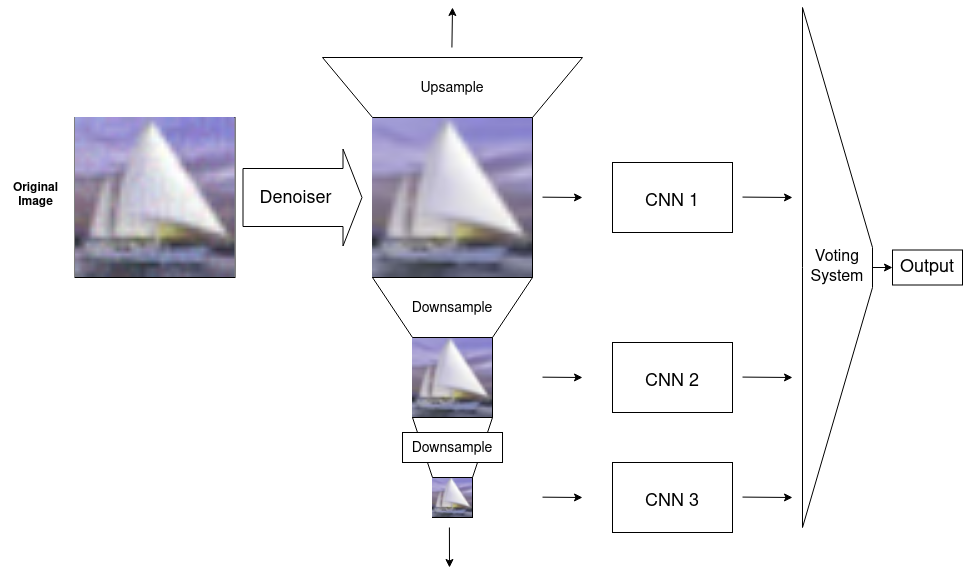
\includegraphics[scale=0.17]{images/diagram.png}
% \caption{Illustration of our proposed method.}
% \end{figure}

\begin{figure}[H]
\centering
    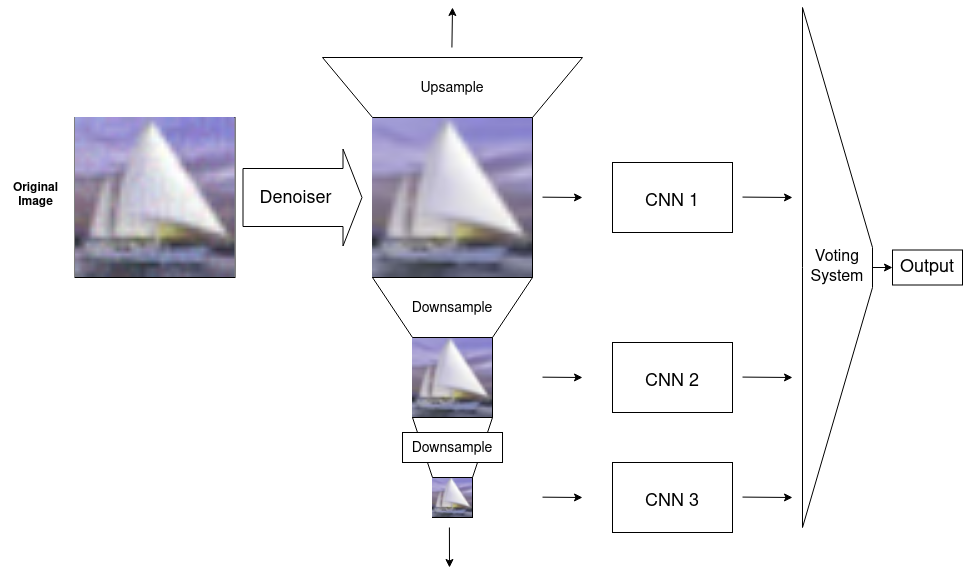
\includegraphics[\columnwidth]{images/diagram.png}
\caption{Illustration of our proposed method.}
\end{figure}

We introduce an ensemble-based defense system where each ensemble member receives a different resized version of the input image from a gaussian pyramid (see Fig. 1). We will experiment with replacing the gaussian blur step with a non-differentiable median filter. With additional time, we also intend to potentially explore using bilinear or median-based upsampling to increase image size, as repeated downsampling will likely destroy image information. 

We also plan on applying a denoiser system before the downscaling process. As seen in recent literature, deep denoisers can be quite effective as a defensive measure. We intend to evaluate the denoising performance of DnCNN compared to no denoising as the baseline. The DnCNN will be trained with a dataset containing adversarial images generated by different attack methods and perturbation levels, which should further improve system robustness. With additional time, we could also compare the denoising performance of the Denoising Autoencoder and U-Net methods. 

In terms of combining the resulting ensemble outputs, we intend to explore the following options:
\begin{itemize}
\item Uniform Average Outputs: A linear baseline.
\item Weighted Average Outputs: Performance scaled weights will likely improve performance on clean inputs, but could lead to targeted attacks on the highest performing models. 
\item Uniform Majority Vote: Equal votes introduces a non-differentiable step.
\item Weighted Majority Vote: Better accuracy on clean inputs, but may be more vulnerable.
\end{itemize}

\section{Experiments and Goals}
We will begin with MNIST and CIFAR10 datasets as most works in the literature do. Then, with enough time, we plan on running our system on ImageNet to examine our system's performance on larger images. We also plan on starting with Resnet 34/50 models, and exploring other model options with additional time. For attacks, we plan on using the cleverhans library in evaluating our system against FGSM, PGD, and C\&W attacks. We leave the SGM attack as a stretch goal. 

For comparison, we plan to run the Ensemble Adversarial Training method and to use a single model vanilla CNN training as a baseline. If we have additional time, we also plan on finding other successful defenses for comparison. 
\section{Timeline}
\begin{itemize}
    \item Nov 19 - Completed literature review.
    \item Nov 24 - Complete implementation of our method. 
    \item Nov 28 - Begin experiments.
    \item Dec 2 - Start preparing Poster and Report.
    \item Dec 4 - Completed experimentation. 
    \item Dec 8 - Project Presentation and Submission
\end{itemize}



\bibliographystyle{IEEEtran}

% \bibliographystyle{plain}
%\bibliography{references}
\begin{thebibliography}{}
 \bibitem[1]{pbba} N. Papernot, P. McDaniel, I. Goodfellow, S. Jha, Z. B. Celik, and A. Swami, “Practical black-box attacks against machine learning,” in Proceedings of the 2017 ACM on Asia conference on computer and communications security, 2017, pp. 506–519.
 \bibitem[2]{fgsm} I. J. Goodfellow, J. Shlens, and C. Szegedy, “Explaining and harnessing adversarial examples,” arXiv preprint arXiv:1412.6572, 2014.
 \bibitem[3]{eat} F. Tramèr, A. Kurakin, N. Papernot, I. Goodfellow, D. Boneh, and P. McDaniel, “Ensemble adversarial training: Attacks and defenses,” arXiv preprint arXiv:1705.07204, 2017.
 \bibitem[4]{pgd} A. Madry, A. Makelov, L. Schmidt, D. Tsipras, and A. Vladu, “Towards deep learning models resistant to adversarial attacks,” arXiv preprint arXiv:1706.06083, 2017.
 \bibitem[5]{cw} N. Carlini and D. Wagner, “Towards evaluating the robustness of neural networks,” in 2017 ieee symposium on security and privacy (sp), 2017, pp. 39–57.
 \bibitem[6]{sgm} D. Wu, Y. Wang, S.-T. Xia, J. Bailey, and X. Ma, “Skip connections matter: On the transferability of adversarial examples generated with resnets,” arXiv preprint arXiv:2002.05990, 2020.
 \bibitem[7]{survey} F. Tramer, N. Carlini, W. Brendel, and A. Madry, “On adaptive attacks to adversarial example defenses,” Advances in Neural Information Processing Systems, vol. 33, pp. 1633–1645, 2020.
 \bibitem[8]{empir} S. Sen, B. Ravindran, and A. Raghunathan, “Empir: Ensembles of mixed precision deep networks for increased robustness against adversarial attacks,” arXiv preprint arXiv:2004.10162, 2020.
 \bibitem[9]{bpda} A. Athalye, N. Carlini, and D. Wagner, “Obfuscated gradients give a false sense of security: Circumventing defenses to adversarial examples,” in International conference on machine learning, 2018, pp. 274–283.
 \bibitem[10]{diversity} T. Pang, K. Xu, C. Du, N. Chen, and J. Zhu, “Improving adversarial robustness via promoting ensemble diversity,” in International Conference on Machine Learning, 2019, pp. 4970–4979.
 \bibitem[11]{cite11} Lee, S., Lee, J., and Park, S. (2018). Defensive denoising methods against adversarial attack. 
 \bibitem[12]{cite12} Maaten, L. V. D., Yuille, A. L., and He, K. (2019). Feature Denoising for Improving Adversarial Robustness. 2019 IEEE/CVF Conference on Computer Vision and Pattern Recognition (CVPR).
 \bibitem[13]{cite13} Bakhti, Y., Fezza, S. A., Hamidouche, W., and Deforges, O. (2019). DDSA: A Defense Against Adversarial Attacks Using Deep Denoising Sparse Autoencoder. IEEE Access, 7, 160397–160407.
 \bibitem[14]{cite14} Liao, F., Liang, M., Dong, Y., Pang, T., Hu, X., and Zhu, J. (2018). Defense Against Adversarial Attacks Using High-Level Representation Guided Denoiser. 2018 IEEE/CVF Conference on Computer Vision and Pattern Recognition.
 \bibitem[15]{cite15} Zuo, W., Chen, Y., Meng, D., and Zhang, L. (2017). Beyond a Gaussian Denoiser: Residual Learning of Deep CNN for Image Denoising. IEEE Transactions on Image Processing, 26(7), 3142–3155.
 
 
\end{thebibliography}



\end{document}


